\section{Method}

In this section, we detail the methodology used to formulate filtering module and determine the discrete integration model
along with the implementation steps to validate our approach.

\subsection{Dataset Description} \label{sec:dataset_descrition}
For our experimentation, we utilized the inD \cite{inDdataset}, exiD \cite{exiDdataset}, and rounD \cite{rounDdataset} datasets provided by the 
\textit{Institut für Kraftfahrzeuge (ika) RWTH Aachen University}.
The datasets offer vehicle trajectories recorded at German intersections, highway exits and entries, 
and roundabouts, respectively. 
Additionally, the datasets were provided with a tool (drone-dataset-tool) \cite{repo:drone-dataset-tool} that allowed us to visualize them for better understanding. 
The datasets include 18 columns, spanning from vehicle identifiers and lifetimes of vehicles to various columns of motion-related data points.

Our analysis primarily targets key data points: 
$x_{\text{Center}}$, $y_{\text{Center}}$, $x_{\text{Velocity}}$, $y_{\text{Velocity}}$, $x_{\text{Acceleration}}$, for the integration model. The filtering module, however, utilizes these columns alongside additional data, allowing for a detailed examination of vehicle dynamics and the identification of specific driving behaviors crucial for enhancing predictive accuracy.

The columns  $x_{\text{Center}}$ and $y_{\text{Center}}$ represent the current position of the object's center in the coordinate coordinate system. Preprocessing was done such that the columns describe the distance to the origin of the vehicle.

Velocity information is captured through columns $x_{\text{Velocity}}$ and $y_{\text{Velocity}}$ representing velocities 
in the x-axis and y-axis respectively.

Acceleration data are represented in columns $x_{\text{Acceleration}}$ and $y_{\text{Acceleration}}$ which provide 
information on the acceleration in the x-axis and y-axis respectively.

For an illustrative example of traffic scenarios and vehicle behaviors captured in the exid and round datasets, see Fig.~\ref{fig:exiD dataset} and Fig.~\ref{fig:rounD dataset}, respectively.

\begin{figure}[h]
    \centering
    \begin{minipage}[b]{0.45\columnwidth}
        \centering
        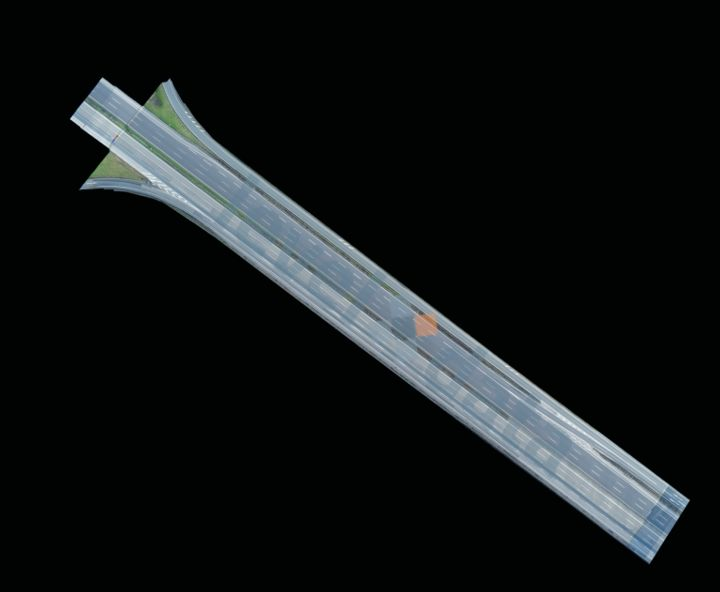
\includegraphics[width=\columnwidth]{images/figures/exid_dataset.jpeg}
        \caption{exiD dataset}
        \label{fig:exiD dataset}
    \end{minipage}
    \hfill
    \begin{minipage}[b]{0.45\columnwidth}
        \centering
        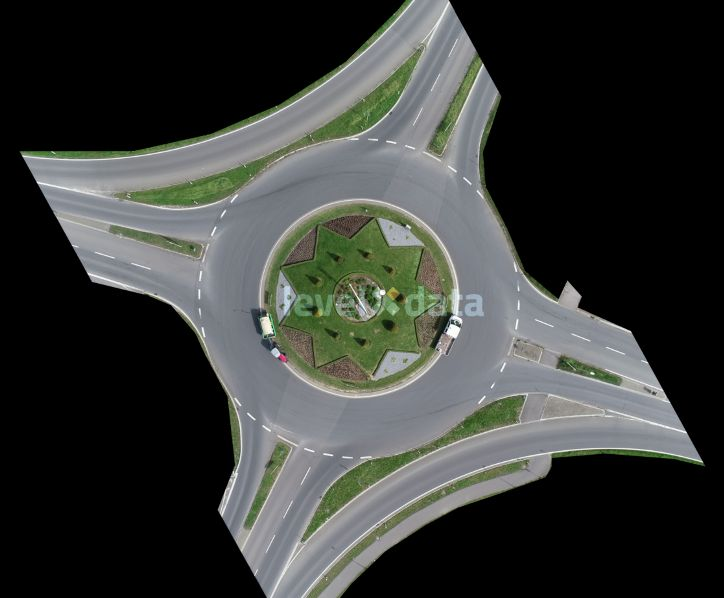
\includegraphics[width=\columnwidth]{images/figures/round_dataset.jpeg}
        \caption{rounD dataset}
        \label{fig:rounD dataset}
    \end{minipage}
\end{figure}

\subsection{Filtering Module} \label{sec:filtering_module}

In addition to the rigorous dataset description already outlined, our methodology incorporates a filtering module designed to refine the datasets further for enhanced predictive modeling. This module, integral to our approach, employs algorithms to process the raw data meticulously, identifying and extracting meaningful patterns indicative of specific vehicle behaviors. These behaviors, crucial for accurate motion prediction, include merging, yielding, and hard braking, among others.

The filtering module operates by first preprocessing the vehicle data to ensure consistency and reliability in the input data. This step involves normalizing the data points to a common reference frame, enabling a more accurate analysis of vehicle trajectories. For instance, the preprocessing involve a transformation formula for normalizing vehicle positions, such as:
\begin{align} 
    \text{Normalized Position} = \frac{\text{Position} - \text{Min Position}}{\text{Max Position} - \text{Min Position}}
\end{align}

Following this, the module applies a series of algorithms aimed at detecting specific behaviors. For instance, the detection of entering vehicles is based on a set of predefined conditions such as interaction distance threshold, relative speed threshold, and yielding behavior, which are crucial for understanding vehicle dynamics at intersections and roundabouts. For detecting entering vehicles and other behaviours, a combination of velocity and acceleration thresholds might be applied, defined as:
\begin{align} 
    \text{Entering Condition} = \left\{
\begin{array}{ll}
\text{True} & \text{if } \Delta v > \text{speed threshold} \\
& \text{and } \Delta d < \text{distance threshold} \\
\text{False} & \text{otherwise}
\end{array}
\right.
\end{align}

Where \(\Delta v\) represents the change in velocity, and \(\Delta d\) signifies the relative distance to another vehicle.


The algorithms within the filtering module make extensive use of the vehicle trajectory data, focusing on parameters such as $x_{\text{Center}}$, $y_{\text{Center}}$, $x_{\text{Velocity}}$, $y_{\text{Velocity}}$, $x_{\text{Acceleration}}$, 
$y_{\text{Acceleration}}$. By analyzing these parameters over time, the module can detect changes in vehicle behavior that signal merging, yielding, or hard braking. This detection is further enhanced by comparing the mean of the first frames (indicative of vehicle entry) and the last frames (indicative of vehicle exit) against established thresholds, thereby identifying vehicles that are entering or exiting the roadway.

Furthermore, the module incorporates functions to detect lane changes, filter vehicles in the same lane, and assess the relative velocity and distance between vehicles to identify potential interactions. These functions are critical for understanding the complex dynamics of vehicle behavior in dense traffic conditions and are instrumental in improving the accuracy of our discrete integration model. For example, lane change detection involves analysing the lateral displacement and comparing it against a lane width parameter to determine if a vehicle has moved sufficiently across lanes:

\begin{align} 
\text{Lane Change Detected} = \left\{
\begin{array}{ll}
\text{True} & \text{if } \left| \Delta x \right| > \frac{\text{Lane Width}}{2} \\
\text{False} & \text{otherwise}
\end{array}
\right.
\end{align}

The module's algorithms also utilize parameters directly from the datasets, such as odrLaneId for lane identification and laneChange flags, to facilitate precise behavioural analyses. These elements are crucial for the module's ability to detect driving behaviours like yielding and hard braking, through the calculation of relative velocities and distances, applying thresholds that have been determined to reflect driving scenarios.

By integrating this filtering module into our methodology, we enhance the quality of the dataset used for modeling. This not only improves the accuracy of our predictive models but also ensures that the models are trained on data that accurately reflect the complexities of real-world driving scenarios. The application of these advanced data processing techniques contributes to the overall robustness and reliability of our approach, setting a new approach for predictive modeling in autonomous driving systems.

\begin{figure}[h]
\centering
\includegraphics[width=\columnwidth]{./images/figures/filtering_module.jpeg}
\caption{Overview of the Filtering Module}
\label{fig:filtering_module}
\end{figure}

The Fig.~\ref{fig:filtering_module} provides a detailed visualization of the structure and functionality of the filtering module, comprising two principal components: Utilities and Interactions Filter. The Utilities package is tasked with the loading and configuration of the dataset, preparing it for analysis. The Interactions Filter, highlighted with an orange bracket, initially focuses on identifying micro behaviors such as speed adjustment and hard braking. It advances to recognize macro behaviors by synthesizing these micro observations, including vehicles' entering, exiting, and overtaking actions. Postprocessing refines the data further, preparing it for the integration module. 

\subsection{Model Selection Process} 
Our model selection process involved a systematic trial and error approach with a total of 8 different models. 
Each model underwent an evaluation process to evaluate its ability to accurately predict vehicle acceleration. 
Ultimately, the following two linear models emerged as the most suitable models
\begin{align} 
    a_{dis}(k) &= \bar{c}_1 \bigl( s(k) - s(k+1) - v(k) \bigr) -\bar{c}_2 a(k-1) \\
    a_{vel}(k) &= \bar{c}_3 \bigl( v(k) - v(k+1) \bigr) -\bar{c}_4 a(k-1) 
\end{align}

These linear models are then solved by linear regression. 
After training the model on the acceleration set from our dataset, we can rearrange the formulas using the newly found coefficients ($\bar c_1,\bar c_2,\bar c_3,\bar c_4$)
to determine the distance and velocity formulas, similar to the ballistic integration
\begin{align} 
    s(k+1) &= s(k) + v(k) + c_1 a_{dis}(k) + c_2 a(k-1) \\
    v(k+1) &= v(k)        + c_3 a_{vel}(k) + c_4 a(k-1)
\end{align}


The coefficients can then be determined through these calculations:
\begin{align}
   c_1 &= \frac{1}{\bar{c}_1} \\
   c_2 &= \bar{c}_2 \cdot c_1 \\
   c_3 &= \frac{1}{\bar{c}_3} \\
   c_4 &= \bar{c}_4 \cdot c_3
\end{align}

By rearranging the model as such, we specifically ensure that for both $s(k)$ and $v(k)$ we receive the same 
acceleration, as we are training both models on the same acceleration set.
Thus, we receive a proper integration method for the data set on which we trained the model on, which solves the 
problems of the mismatched acceleration in previous attempts.
As seen in the section \ref{sec:dataset_descrition}, we can see, that the columns for distance, velocity and acceleration are 
split into their x- and y-components.
Our linear models will look like this:

\hfil

\textbf{Distance Model} (Acceleration from distance formula):
{\footnotesize
\begin{align} \label{eq:lin_model_acc_dis}
    \begin{bmatrix}
        a_x(k) \\ 
        a_y(k)       
    \end{bmatrix}_{\text{dis}}
    =
    \begin{bmatrix}
       s_x(k) - s_x(k+1) - v_x(k) & -a_x(k-1) \\ 
       s_y(k) - s_y(k+1) - v_y(k) & -a_y(k-1)   
    \end{bmatrix}
    \begin{bmatrix}
        \overline{c}_1 \\
        \overline{c}_2 \\
   \end{bmatrix}
\end{align}
}

\textbf{Velocity Model} (Acceleration from velocity formula):
\begin{align} \label{eq:lin_model_acc_vel}
    \begin{bmatrix}
        a_x(k) \\ 
        a_y(k) 
    \end{bmatrix}_{\text{vel}}
    =
    \begin{bmatrix}
        v_x(k) - v_x(k+1) & -a_x(k+1)    \\ 
        v_y(k) - v_y(k+1) & -a_y(k+1)    \\
    \end{bmatrix}
    \begin{bmatrix}
        \overline{c}_3 \\
        \overline{c}_4 \\
   \end{bmatrix}
\end{align}

\hfil

Afterward, we will compare the accelerations derived from displacement, denoted as 
$\begin{bmatrix} a_x(k) \\ a_y(k) \end{bmatrix}_{dis}$
, with those derived from velocity, denoted as 
$\begin{bmatrix} a_x(k) \\ a_y(k) \end{bmatrix}_{\text{vel}}$
, to assess the effectiveness of the distance model's acceleration estimation relative to that of the velocity model.


Using the coefficients determined from linear regression from the linear models \eqref{eq:lin_model_acc_dis} 
and \eqref{eq:lin_model_acc_vel}, we can determine the distance and velocity using the following 
matrices:

\hfil

\textbf{Distance formula}
{\footnotesize
\begin{align}
\label{eq:distance_matrix}
    \begin{bmatrix} s_x(k+1) \\ s_y(k+1) \end{bmatrix}
    =
    \begin{bmatrix} a_x(k) & a_x(k-1)    \\ a_y(k) & a_y(k-1)    \\ \end{bmatrix}
    \begin{bmatrix} c_1 \\ c_2 \\ \end{bmatrix}
    +
    \begin{bmatrix} s_x(k) + v_x(k) \\ s_y(k) + v_y(k) \\ \end{bmatrix}
\end{align} 
}

\hfil

\textbf{Velocity formula}
\begin{align}
\label{eq:velocity_matrix}
    \begin{bmatrix} v_x(k+1) \\ v_y(k+1) \end{bmatrix}
    =
    \begin{bmatrix} a_x(k) & a_x(k-1)    \\ a_y(k) & a_y(k-1)    \\ \end{bmatrix}
    \begin{bmatrix} c_3 \\ c_4 \\ \end{bmatrix}
    +
    \begin{bmatrix} v_x(k) \\ v_y(k) \end{bmatrix}
\end{align}


Hence, we obtain a discrete integration model with matching accelerations for the distance and velocity formula. For a detailed visualization of the integration module's pipeline, including how these coefficients are applied within the broader framework of our model, please refer to Fig.~\ref{fig:filtering_module} below.

\begin{figure}[h]
\centering
\includegraphics[width=\columnwidth]{./images/figures/integration_module.png}
\caption{Overview of the Integration Module}
\label{fig:Integration_module}
\end{figure}


\subsection{Evaluation Metrics and Results}

The evaluation of our linear model's performance relies on the following metrics for linear regression: Mean Squared Error (MSE), Mean Absolute Error (MAE), and R-squared ($R^2$) score.

Mean Squared Error (MSE) measures the average squared difference between the actual and predicted values. It penalizes large errors more heavily than smaller ones, making it sensitive to outliers. A lower MSE indicates better model performance.

Mean Absolute Error (MAE) calculates the average absolute difference between the actual and predicted values and is
not affected by the scale of the data. Like MSE, lower MAE values indicate better model performance.

R-squared ($R^2$) score quantifies the proportion of the variance in the dependent variable that is predictable 
from the independent variables. 
It ranges from 0 to 1, where a value closer to 1 indicates a better fit of the model to the data. 

